\section{Returning to the Z1 support: complete prime clocks, loops, and
zeta
characters}\label{returning-to-the-z1-support-complete-prime-clocks-loops-and-zeta-characters}

24 September 2026. Proofs PL1--PL8. This calculation tests the user's
proposed mechanism: a deformation invisible to the complete counting
system should be a change of clock, or a loop whose return might expose
the distinguished presence support. The comparison is made on the actual
reconstructed arithmetic, the Connes--Consani prime curves, and the
original zeta function.

The notation is retained: \(Z_0\) is absence; \(Z_1\) is primitive
presence \(\tau\), without \(Z_2\) parity. No addition, coordinate,
metric, or winding number is assigned to \(\tau\). The previously proved
supporting role of \(\tau\langle Z_1;\mathrm{no}\ Z_2\rangle\) is the
common point \(\eta\). The stalk, its winding quotient, and its
arithmetic endomorphisms remain part of the complete datum.

\subsection{PL1. What the complete counting reconstruction already
fixes}\label{pl1.-what-the-complete-counting-reconstruction-already-fixes}

The source contains the signed monomial group \[
G=\langle T,J,\epsilon:\ TJ=JT,\ T\epsilon=\epsilon T,\
J\epsilon=\epsilon J,\ J^2=\epsilon,\ \epsilon^2=1\rangle
\cong\mathbb Z\times C_4,
\] its finite subgroup \(H=\langle J\rangle\), and the infinite cyclic
winding group \(W=G/H\). The separate absorbing source element is
outside this group and is not identified with its identity. The exact
sequence, source involution and both chart maps are retained in
CG2--CG4: \[
1\longrightarrow H\longrightarrow G\longrightarrow W\longrightarrow1,
\quad A(T)=\epsilon T^{-1},\quad A(J)=J^{-1}.
\tag{PL1.1}
\] The arithmetic ring is \(R=\operatorname{End}_{\mathrm{Ab}}(W)\),
with pointwise group multiplication as its addition and composition as
its multiplication. Every endomorphism is the power map \([n]\),
independently of the choice of generator of \(W\). Thus \[
R\cong\mathbb Z,\qquad \mathbf1_R=\operatorname{id}_W,\qquad
[a]+[b]=[a+b],\quad [a][b]=[ab].
\tag{PL1.2}
\] These are operations on endomorphisms, not on \(\tau\). Any unital
ring automorphism of this reconstructed \(R\) is the identity: it fixes
\(\mathbf1_R\), hence each of its finite sums, their additive inverses,
and therefore every \([n]\). Consequently it fixes every prime ideal and
its residue norm \(p=|W/[p]W|\).

Retain all three complete measures: \[
\mathcal R=\sum_p\sum_{k\ge1}\frac1k\delta_{k\log p},\quad
\mathcal D=\delta_0+\sum_{n\ge2}\delta_{\log n}=\exp_*\mathcal R,\quad
\mathcal W=\sum_p\sum_{k\ge1}(\log p)\delta_{k\log p}=t\mathcal R.
\tag{PL1.3}
\] TP9--TP13 and IH1 prove these locally finite measure identities with
all coefficients and the unit atom retained. Their transforms on
\(\Re s>1\) are the original functions \[
\int e^{-st}d\mathcal D(t)=\zeta(s),\qquad
\int e^{-st}d\mathcal W(t)=-\frac{\zeta'(s)}{\zeta(s)}.
\tag{PL1.4}
\] The composed CG/I26 proof identifies the same meromorphic zeta
function and zero multiplicities in both charts. That identification is
closed in this route.

\subsection{PL2. An invisible change of clock cannot turn an
off-critical zero into a critical
one}\label{pl2.-an-invisible-change-of-clock-cannot-turn-an-off-critical-zero-into-a-critical-one}

Specify the proposed clock change. Let \(h:\mathbb R\to\mathbb R\) be an
order-preserving bijection that preserves composition of logarithmic
durations and the identity duration: \[
h(t+u)=h(t)+h(u),\qquad h(0)=0.
\tag{PL2.1}
\] Then \(h(t)=ct\) for a unique \(c>0\). Indeed \(c=h(1)>0\);
additivity gives \(h(a/b)=ca/b\) for every rational \(a/b\). Rational
lower and upper approximations to a real \(t\), together with
monotonicity, force \(h(t)=ct\). There is no nonlinear bending in this
stated class. A translation by \(b\) preserves (PL2.1) only when
\(b=0\).

This proof states exactly what is preserved; it does not classify every
transformation of every space merely from the word ``invisible.'' On the
full normed arithmetic with the specified times \(t_p=\log p\),
preserving even one such time forces \(c=1\). A simultaneous change of
measuring units remains a valid comparison, with every factor as
follows. Write \(S_c(t)=ct\): \[
\mathcal D_c=(S_c)_*\mathcal D,\qquad
\mathcal R_c=(S_c)_*\mathcal R,\qquad
\mathcal W_c=t\mathcal R_c=c(S_c)_*\mathcal W.
\tag{PL2.2}
\] For \(\Re(cs)>1\), \[
\int e^{-st}d\mathcal D_c(t)=\zeta(cs),\qquad
\int e^{-st}d\mathcal W_c(t)
=-c\,\frac{\zeta'(cs)}{\zeta(cs)}.
\tag{PL2.3}
\] The factor \(c\) in the second equality comes from the rescaled
primitive return length. The pole, its residue, the nontrivial zeros,
and the trivial zeros become \[
\frac1c,\quad\frac1c,\quad\frac{\rho}{c},\quad-\frac{2r}{c}\ (r\ge1).
\tag{PL2.4}
\] Zero multiplicities are unchanged. The exact comparison with a
completed object, without adopting it as the working object, is \[
\xi(cs)=\frac12(cs)(cs-1)\pi^{-cs/2}\Gamma(cs/2)\zeta(cs).
\tag{PL2.5}
\] Its derivative retains all contributions: \[
c\frac{\xi'(cs)}{\xi(cs)}
=c\frac{\zeta'(cs)}{\zeta(cs)}+\frac1s+\frac{c}{cs-1}
-\frac c2\log\pi+\frac c2\frac{\Gamma'(cs/2)}{\Gamma(cs/2)}.
\tag{PL2.6}
\] The reflection becomes \(s\mapsto c^{-1}-s\). Hence the critical line
has real coordinate \(1/(2c)\), and \[
2\Re(\rho/c)-1/c=(2\Re\rho-1)/c.
\tag{PL2.7}
\] A change of clock therefore cannot hide or manufacture
off-criticality: it rescales the zero and the comparison line together.
This proves the proposed dilation invariance for the complete original
function, including its exceptional points.

\subsection{PL3. All prime curves together: no positive real period, and
the angular loop
survives}\label{pl3.-all-prime-curves-together-no-positive-real-period-and-the-angular-loop-survives}

The original Connes--Consani curve is \[
E_p=\mathbb C^\times/p^\mathbb Z.
\tag{PL3.1}
\] Their exponential coordinate is \(z=\exp(2\pi i w)\), with periods
\(1\) and \(i\log p/(2\pi)\). To work directly with the original
differential \(dz/z\), retain the exact comparison \(u=2\pi i w\). The
two oriented periods become \(2\pi i\) and \(-\log p\); the lattice as a
subgroup is \[
\Lambda_p^{\log}=2\pi i\mathbb Z+(\log p)\mathbb Z,\qquad
\frac{dz}{z}=du.
\tag{PL3.2}
\] The sign of the second oriented source generator has been exhibited.
The source's modular parameter is a parameter of \(E_p\), not the user's
primitive \(\tau\).

For the positive real flow \(t\mapsto[e^t]_p\), return occurs precisely
when \(t=k\log p\), \(k\in\mathbb Z\). Use the joint map \[
\jmath_{\mathbb R}:\mathbb R\longrightarrow E_2\times E_3,\qquad
t\longmapsto([e^t]_2,[e^t]_3).
\tag{PL3.3}
\] Its kernel is zero: \(t=a\log2=b\log3\) would imply \(2^a=3^b\);
clearing negative exponents and unique factorization give \(a=b=0\).
Therefore the joint real clock cannot return to its starting state at a
nonzero time even though each individual prime orbit is a circle.
Keeping more primes cannot enlarge this kernel.

There is nevertheless a genuine common angular period: \[
\Lambda_2^{\log}\cap\Lambda_3^{\log}=2\pi i\mathbb Z.
\tag{PL3.4}
\] Equality of two lattice elements forces their real parts to vanish by
the preceding proof; their imaginary parts leave precisely the stated
integer multiples. The exact map \[
\jmath_{\mathbb C^\times}:\mathbb C^\times\longrightarrow E_2\times E_3,
\qquad z\longmapsto([z]_2,[z]_3)
\tag{PL3.5}
\] is injective, since its kernel is
\(2^\mathbb Z\cap3^\mathbb Z=\{1\}\).

Injectivity is the assertion here; no topological embedding into the
compact product is asserted. The angular loop has not been suppressed by
considering only positive real time. It is the original exponential
covering period, present before any question about zeta zeros.

\subsection{PL4. Returning to the same Z1 support does not identify the
retained
winding}\label{pl4.-returning-to-the-same-z1-support-does-not-identify-the-retained-winding}

The actual source space is \[
X=\{+,-,\eta\},\quad
\Omega_+=\{+,\eta\},\quad\Omega_-=\{-,\eta\},\quad
\Omega_+\cap\Omega_-=\{\eta\}.
\tag{PL4.1}
\] The projection of the generic monomials to their support is the set
map \[
\pi:G\longrightarrow\{\eta\},\qquad \pi(T^mJ^k)=\eta.
\tag{PL4.2}
\] Every winding has the same supporting point under this map. Its fibre
is the entire \(G\), including all four \(J\)-states and all integer
windings. Thus seeing the \(Z_1\) support again does not, by this
observation alone, mean that the full state has returned. This is a
direct calculation of the map and its fibre; it neither assigns parity
to \(\tau\) nor identifies different monomials.

An actual identification of winding after \(N>0\) steps is the quotient
\[
q_N:W\longrightarrow W/NW,\qquad \ker q_N=NW.
\tag{PL4.3}
\] It acts on reconstructed arithmetic by \[
R\longrightarrow\operatorname{End}(W/NW)\cong\mathbb Z/N\mathbb Z,\qquad
[n]\longmapsto[n\bmod N].
\tag{PL4.4}
\] The kernel is \(N\mathbb Z\): an endomorphism vanishes on the
quotient exactly when its degree is divisible by \(N\). Thus the loop is
detected by the lost endomorphisms. This zero is a receiver's zero
endomorphism, not source absence.

On the full signed group, the quotient \(G/\langle T^N\rangle\)
preserves the original involution \(A\) exactly when \(N\) is even.
Indeed \(A(T^N)=\epsilon^NT^{-N}\), whose class is the identity
precisely when \(\epsilon^N=1\), since all four \(J\)-states remain. Odd
\(N\) would require additionally killing \(\epsilon\), changing the
specified signed datum. Using every even \(N\) retains the full datum
faithfully: if \(T^mJ^k\) maps to the identity in every such quotient,
then \(J^k=1\) and every even \(N\) divides \(m\); choosing even
\(N>|m|\) forces \(m=0\).

These exact quotients identify the information that closed winding
loses. They also show why many individually periodic observations can
jointly retain an infinite clock.

\subsection{PL5. Folding the complete absorption record around a circle
is
detectable}\label{pl5.-folding-the-complete-absorption-record-around-a-circle-is-detectable}

Let \(L>0\), \(C_L=\mathbb R/L\mathbb Z\), and \(q_L(t)=t\bmod L\).
Pushforward gives actual measures: \[
(q_L)_*\mathcal D=\sum_{n\ge1}\delta_{\log n\bmod L},\qquad
(q_L)_*\mathcal W=\sum_{p,k\ge1}(\log p)\delta_{k\log p\bmod L}.
\tag{PL5.1}
\] Both give infinite mass to every nonempty open arc. For the first,
lift an arc to \(a<t<b\), \(b-a<L\). The disjoint intervals
\((e^{a+jL},e^{b+jL})\), for sufficiently large positive \(j\), each
contain an integer. Each gives an atom in that arc, proving infinite
mass.

For the second, at least one of \(\log2/L,\log3/L\) is irrational,
because otherwise \(\log2/\log3\) would be rational. Positive multiples
of an irrational circle rotation visit every open arc infinitely often.
To justify the needed fact, pigeonhole \(M+1\) successive multiples into
\(M\) equal arcs, giving a nonzero multiple within \(L/M\) of zero in
the circle metric. These distances become arbitrarily small, so the
closed subgroup generated by the rotation is the whole circle: multiples
of a sufficiently small positive representative approximate every circle
point. Positive multiples have the same closure. A subsequence of
positive multiples tends to zero, and subtracting any fixed multiple
from sufficiently late terms approximates its negative using positive
multiples. Every tail of the positive orbit is therefore dense. Each
visit contributes the fixed positive weight \(\log p\), proving the
assertion.

The folded unweighted record is consequently not locally finite, unlike
the original record on bounded real intervals. The pushforward still
exists as a measure; it has not become the same counting object.

There is an exact finite comparison retaining every convergence factor.
For \(\sigma>1\), set \[
\mathcal D_{\sigma,L}=(q_L)_*(e^{-\sigma t}\mathcal D),\qquad
\mathcal W_{\sigma,L}=(q_L)_*(e^{-\sigma t}\mathcal W).
\] Their circle Fourier coefficients, with kernel \(e^{-2\pi i jt/L}\),
are \[
\widehat{\mathcal D_{\sigma,L}}(j)
=\zeta(\sigma+2\pi i j/L),\qquad
\widehat{\mathcal W_{\sigma,L}}(j)
=-\frac{\zeta'(\sigma+2\pi i j/L)}{\zeta(\sigma+2\pi i j/L)}.
\tag{PL5.2}
\] Absolute convergence proves both identities by substitution into
(PL1.4). The explicit weight has not replaced the unweighted object.

For the existing prime circle \(L=\log p\), the mass at its identity is
\[
\mathcal D_{\sigma,\log p}(\{0\})
=\sum_{k\ge0}p^{-k\sigma}=\frac1{1-p^{-\sigma}}>1,
\tag{PL5.3}
\] whereas the original unit atom has mass one. The corresponding
prime-power mass is \[
\mathcal W_{\sigma,\log p}(\{0\})
=(\log p)\sum_{k\ge1}p^{-k\sigma}
=\frac{\log p}{p^\sigma-1}>0.
\tag{PL5.4}
\] No other prime contributes at this identity: \(q^k=p^a\) forces
\(q=p\). The programme retains these repetitions instead of erasing them
when a point returns.

Checking only the origin is insufficient even for these exact quotients.
For \(L=\log(3/2)\), the images of integer events 2 and 3 coincide,
while the only integer sent to the origin is 1. Indeed a collision is
exactly \(\log(n/m)\in L\mathbb Z\), and an integer at the origin would
be \((3/2)^j\). Unique factorization excludes this being an integer for
any nonzero integer \(j\). This quotient is excluded by the complete
count precisely because it identifies two prime events, even though the
unit observation alone does not expose it. It is not a counterexample to
the complete reconstruction.

\subsection{PL6. What a zero contributes to a loop: a return
multiplier}\label{pl6.-what-a-zero-contributes-to-a-loop-a-return-multiplier}

The actual quotient \(Q\), Mellin observations and maps \(W_a\) are
constructed with full formulas in IH2--IH3. For an actual zeta zero
\(\rho=\beta+i\gamma\), the observation is a character satisfying \[
F_{W_aq}(\rho)=a^\rho F_q(\rho),\qquad
a^\rho=e^{\rho\log a},\qquad a>0.
\tag{PL6.1}
\] This acts on observed amplitudes. It does not replace the prime norm
\(p\) by \(p^\rho\), permute primes, or move an event \(k\log p\). Its
exact relation to the clock is the character identity
\((ab)^\rho=a^\rho b^\rho\).

On the real universal cover of \(C_L\), \(v_\rho(t)=e^{\rho t}\) obeys
\[
v_\rho(t+L)=e^{\rho L}v_\rho(t).
\tag{PL6.2}
\] It descends to an ordinary scalar function on \(C_L\) exactly when
\(e^{\rho L}=1\). For a nontrivial zero, \(0<\beta<1\), so
\(|e^{\rho L}|=e^{\beta L}>1\); scalar descent fails for critical-line
zeros as well as off-critical ones.

An exact receiving object retains the character. On the trivial complex
line bundle over \(C_L\), the one-form \(dt\) is globally defined and \[
\nabla_\rho=d-\rho\,dt
\tag{PL6.3}
\] is a well-defined connection. Its horizontal equation is
\(dv/dt=\rho v\); transport around the positively oriented circle
multiplies the fibre by \(e^{\rho L}\). On
\(E_p=\mathbb C/\Lambda_p^{\log}\), the connection \(d-\rho\,du\) has
multipliers \[
p^\rho,\qquad e^{2\pi i\rho}
\tag{PL6.4}
\] along the positive real and positive angular periods. Both remain.
This line bundle with connection is constructed for each character; no
identification with all source cohomology is assumed. It proves how the
loop and the actual spectral character are related.

At a prime the weight-one comparison is \[
|p^\rho|^2-p=p^{2\beta}-p.
\tag{PL6.5}
\] At \(\beta=1/2\), a full return still multiplies a nonzero vector by
\(p^{1/2+i\gamma}\), not by one; its squared magnitude agrees with
arithmetic degree \(p\). At \(\beta\ne1/2\), the same complete degree
record remains \(p\), while this equality fails. This tests fibre
transport relative to degree, not whether the support has appeared
again.

The common angular period has transport \[
|e^{2\pi i\rho}|=e^{-2\pi\gamma}.
\tag{PL6.6}
\] It does not distinguish \(\beta=1/2\) from another \(\beta\). The
retained angular loop therefore cannot be relabelled as an
off-critical-only phenomenon.

For multiplicity \(m\), retain the full primary block: \[
p^{\rho+t_\rho}
=p^\rho\sum_{r=0}^{m-1}\frac{(\log p)^r}{r!}t_\rho^r,\qquad
e^{2\pi i(\rho+t_\rho)}
=e^{2\pi i\rho}\sum_{r=0}^{m-1}\frac{(2\pi i)^r}{r!}t_\rho^r
\quad\bmod t_\rho^m.
\tag{PL6.7}
\] These solve the same constant-coefficient connection with coefficient
\(\rho+t_\rho\). No nilpotent or repeated-zero datum is omitted.

The full complex reflection also has an exact map. Denote the line with
connection \(d-\rho\,du\) by \(\mathscr K_{\rho,p}\), and let
\(c_p:E_p\to E_p\) be \([u]\mapsto[\overline u]\). This is well defined
because conjugation preserves the lattice. With
\(\rho^\#=1-\overline\rho\), multiplication on the one-dimensional
fibres gives \[
c_p^*\overline{\mathscr K_{\rho,p}}\otimes\mathscr K_{\rho^\#,p}
\ \cong\ \mathscr K_{1,p}.
\tag{PL6.8}
\] To check the connection, pullback after conjugation sends its
coefficient to \(\overline\rho\,du\). The tensor connection is therefore
\(d-(\overline\rho+1-\overline\rho)du=d-du\). Equivalently its
multiplier around any \(\lambda\in\Lambda_p^{\log}\) is
\(e^{\overline\rho\lambda}e^{(1-\overline\rho)\lambda}=e^\lambda\). This
includes the angular period, where it equals one. Omitting the base
conjugation would give \(\overline\lambda\) in the first factor and
would generally fail on that period. This duality holds for off-critical
pairs too; it is not by itself a positive Hermitian norm on one of their
fibres.

\subsection{PL7. What a hypothetical off-critical zero is composed
from}\label{pl7.-what-a-hypothetical-off-critical-zero-is-composed-from}

The original zeta has the exact expression, for \(0<\Re s<1\), \[
\zeta(s)=\frac{\displaystyle\sum_{n=1}^{\infty}(-1)^{n-1}n^{-s}}
{1-2^{1-s}}.
\tag{PL7.1}
\] Every \(n\), its parity sign, and \(\log n\) come from the
reconstructed arithmetic. No parity or addition on \(\tau\) is used.
Here is the derivation, keeping zeta rather than replacing it by the
numerator.

On \(\Re s>1\), separating even terms in the absolutely convergent
original series gives numerator \(=(1-2^{1-s})\zeta(s)\). For
\(\Re s=\sigma>0\), pair consecutive terms: \[
(2k-1)^{-s}-(2k)^{-s}
=s\int_{2k-1}^{2k}x^{-s-1}\,dx.
\] The paired series converges absolutely, locally uniformly in this
half-plane. Its unpaired last term tends to zero. Hence the numerator is
holomorphic there and agrees with the displayed product by analytic
continuation. In \(0<\Re s<1\), the denominator cannot vanish because
\(|2^{1-s}|=2^{1-\Re s}>1\). This proves (PL7.1) on the required domain.
The classical identity is also
\href{https://dlmf.nist.gov/25.2\#E3}{DLMF 25.2.3}.

For an actual zero \(\rho=\beta+i\gamma\), (PL7.1) is exactly the two
cancellation equations \[
\sum_{n\ge1}(-1)^{n-1}n^{-\beta}\cos(\gamma\log n)=0,\qquad
\sum_{n\ge1}(-1)^{n-1}n^{-\beta}\sin(\gamma\log n)=0.
\tag{PL7.2}
\] The series retain their increasing integer order, justified above.
The imaginary part of \(n^{-\rho}\) has a minus sign; setting it to zero
yields the second equation displayed. These equations change none of the
counted integers. They specify a property of the uniquely reconstructed
function.

The complete absorption identity, derived with all Gamma and endpoint
terms in IH4, is \[
\mathcal W=e^t\,dt-\sum_\omega m_\omega e^{\omega t}\,dt
-\sum_{r\ge1}e^{-2rt}\,dt
\quad\text{on }C_c^\infty((0,\infty)).
\tag{PL7.3}
\] This is a distributional identity on these smooth tests, not a
pointwise density series. An off-critical orbit
\(\{\rho,1-\overline\rho,\overline\rho,1-\rho\}\) of common multiplicity
\(m\) contributes \[
-2m\bigl(e^{\beta t}+e^{(1-\beta)t}\bigr)\cos(\gamma t).
\tag{PL7.4}
\] The prime record on the left is unchanged. The exponents describe
cancellation within that record's spectral formula, not a second
candidate prime record with altered event times. A single spectral
summand is not separately equal to a positive counting measure.

An explicit detector exists inside the actual quotient. Choose a
nonnegative nonzero smooth compactly supported \(\varphi(v)\) and set \[
k_\rho(e^v)=\varphi(v)e^{-(\rho-1/2)v}.
\] Then \(F_{k_\rho}(\rho)=\int\varphi(v)\,dv>0\), whereas the defining
ideal of the quotient has zero observation at \(\rho\). IH6 also
constructs one faithful receiver for all reduced observations through
the complete signed grid \(a\log2+b\log3\), \(a,b\in\mathbb Z\),
retaining every other prime action by continuous translation.

\subsection{PL8. Outcome of the proposed loop
contradiction}\label{pl8.-outcome-of-the-proposed-loop-contradiction}

The calculation gives definite exclusions: simultaneous rescaling
preserves off-criticality relative to the pole and reflection; a
nonlinear order- and composition-preserving clock change does not exist;
a nonzero common positive real return does not exist; and forgetting
winding has an explicit detectable kernel. The existing common angular
loop and every local prime loop remain, with their exact return maps.

These results exclude the proposed invisible clock changes. They do not
force a zeta zero to be such a change. Its actual map is (PL6.1), and
its defining equation is (PL7.2), both on the already reconstructed
arithmetic. Reappearance of the \(Z_1\) support alone records (PL4.2);
fibre transport is additional retained data calculated in
(PL6.4)--(PL6.7). No contradiction follows from reappearance alone.

The quantity testing the stronger return comparison is \(p^{2\beta}-p\),
with multiplicity blocks and all-prime compatibility retained. This note
calculates it and the surrounding maps; it does not prove that it
vanishes for all actual zeros or exhibit an actual off-critical zero.
The scalar original-zeta identification remains proved; RH is neither
proved nor disproved here.

\begin{figure}
\centering
\pandocbounded{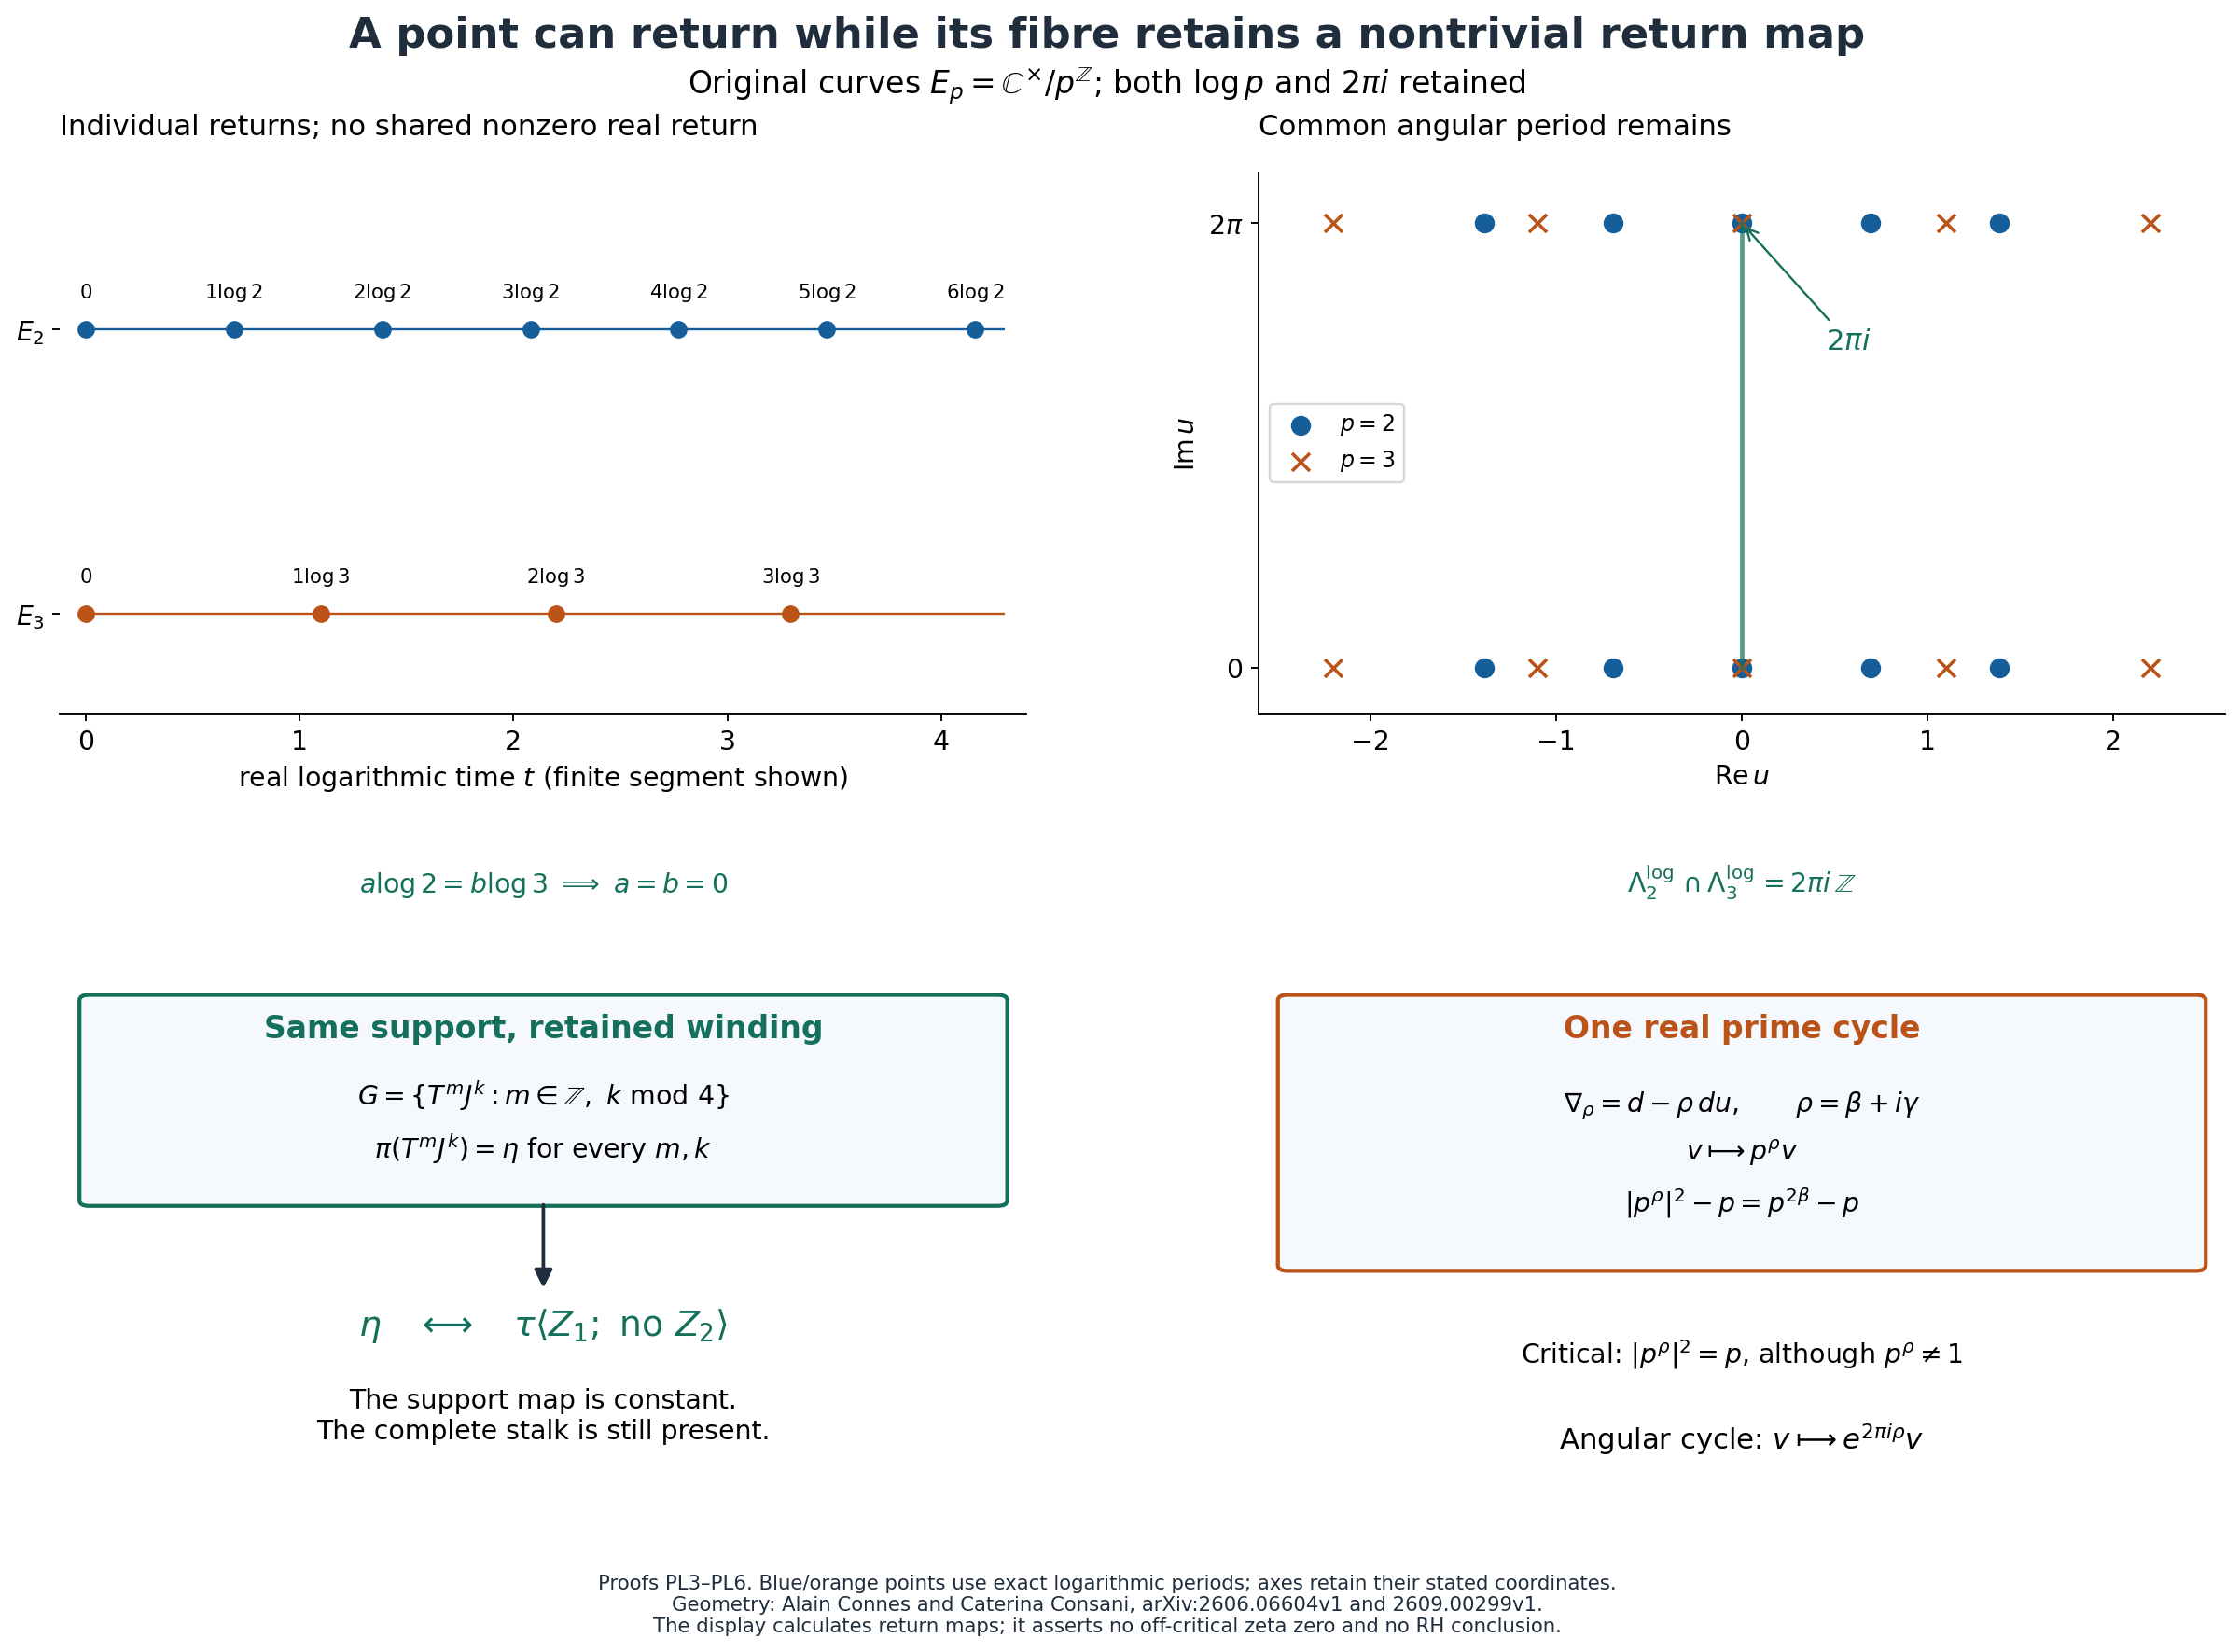
\includegraphics[keepaspectratio,alt={Complete clocks, common angular loop, and fibre return}]{integrality_purity_20260924/PRIME_CLOCK_LOOPS_AND_Z1.png}}
\caption{Complete clocks, common angular loop, and fibre return}
\end{figure}

Figure: exact maps in PL2--PL6, retaining original periods \(\log p\)
and \(2\pi i\). The pictured two-clock orbit is a finite segment; its
no-return assertion is proved in PL3. The occurrence of \(\eta\) labels
source support, not a numerical position. Reproducible figure sources
accompany the proof.

\subsection{Sources and provenance}\label{sources-and-provenance}

Human geometry: Alain Connes and Caterina Consani,
\href{https://arxiv.org/abs/2609.00299v1}{The Absolute Twistor Line and
the Geometry of the compactification of Spec Z, arXiv:2609.00299v1},
original author CC.tex, labels opens1, opens, eq:restriction\_maps,
lines 499--600; and \href{https://arxiv.org/abs/2606.06604v1}{On the
Absolute Geometry of Spec Z and the Fargues--Fontaine curve,
arXiv:2606.06604v1}, original author FF.tex, lines 1550--1633, including
thm:tate\_decomposition. These passages were read directly in the
original TeX. The periods, original coordinate and decomposition
\(E_p=C_p\times S^1\) are their results; the joint-period and return
comparisons are derived here.

Programme sources: CG0--CG8 in \nolinkurl{CANONICAL_GENERIC_RECONSTRUCTION.md};
I26.1--I26.4 in \nolinkurl{ITEM26_CANONICAL_ZETA_COMPOSITION.md};
\href{https://github.com/KokunoYumeto/zeta-function-research-reader/blob/32acd0df89ae22c96d2bc30372e4426a31ce4506/workbenches/splitzero-tandem/temporary-arguments/20260924-fixed-generic-point-purity/timed-prime-reconstruction/README.md}{TP0--TP14
public proof, pinned edition}; and the complete accompanying IH1--IH8
proof. The private reading ledger records actual ranges and versions;
this is not a claim to have reread every programme source in full.

The user supplied the global counting, dilation and returning-support
questions. The classifications and maps above are receiving
calculations, independently compared with the integrality/prime-action
agent's derivation. No historical novelty is claimed for elementary
clock or covering arguments. No new remote publication receipt is
claimed.
